

The following is mostly borrowed from the Wikipedia page on multigrid methods\footnote{\url{https://en.wikipedia.org/wiki/Multigrid_method}}.

There are many types of (geometric) multigrid algorithms, but the common features are that a hierarchy of grids is considered. The important steps are:

\begin{itemize}
\item {\sl Smoothing}: reducing high frequency errors, for example using a few iterations of the Gauss-Seidel method.
\item {\sl Residual Computation}: computing residual error after the smoothing operation(s).
\item {\sl Restriction}: downsampling the residual error to a coarser grid.
\item {\sl Interpolation or prolongation}: interpolating a correction computed on a coarser grid into a finer grid.
\item {\sl Correction}: Adding prolongated coarser grid solution onto the finer grid.
\end{itemize}

There are many choices of multigrid methods with varying trade-offs between speed of solving a single iteration and the rate of convergence with said iteration. The 3 main types are V-Cycle, F-Cycle, and W-Cycle.

Any geometric multigrid cycle iteration is performed on a hierarchy of grids and hence it can be coded using recursion. Since the function calls itself with smaller sized (coarser) parameters, the coarsest grid is where the recursion stops.

Note that the ratio of the number of nodes between two consecutive levels has to be constant between all the levels. Often powers of 2 are used (especially if the grids are based on quad/octrees) but it is not a requirement. 



\begin{center}
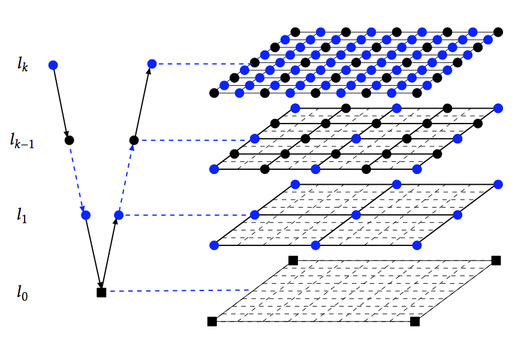
\includegraphics[width=6cm]{images/multigrid/mggrid}\\
{\scriptsize Image from \url{http://web.utk.edu/~wfeng1/research.html}}
\end{center}



What follows is a pseudo-code example of a recursive V-Cycle Multigrid for solving 
the Poisson equation ($\nabla^2 \phi = f$) 
on a uniform grid of spacing $h$:

\begin{verbatim}
function phi = V_Cycle(phi,f,h)
% Pre-Smoothing
phi = smoothing(phi,f,h);
% Compute Residual Errors
r = residual(phi,f,h);
% Restriction
rhs = restriction(r);
eps = zeros(size(rhs));
% stop recursion at smallest grid size
if smallest_grid_size_is_achieved
   eps = smoothing(eps,rhs,2*h);
else        
   eps = V_Cycle(eps,rhs,2*h);        
end
% Prolongation and Correction
phi = phi + prolongation(eps);
% Post-Smoothing
phi = smoothing(phi,f,h);    
end
\end{verbatim}

A multigrid method with an intentionally reduced tolerance can be used as an efficient preconditioner for an external iterative solver. The solution may still be obtained in ${\cal O}(N)$ time as well as in the case where the multigrid method is used as a solver. Multigrid preconditioning is used in practice even for linear systems, typically with one cycle per iteration.

\begin{center}
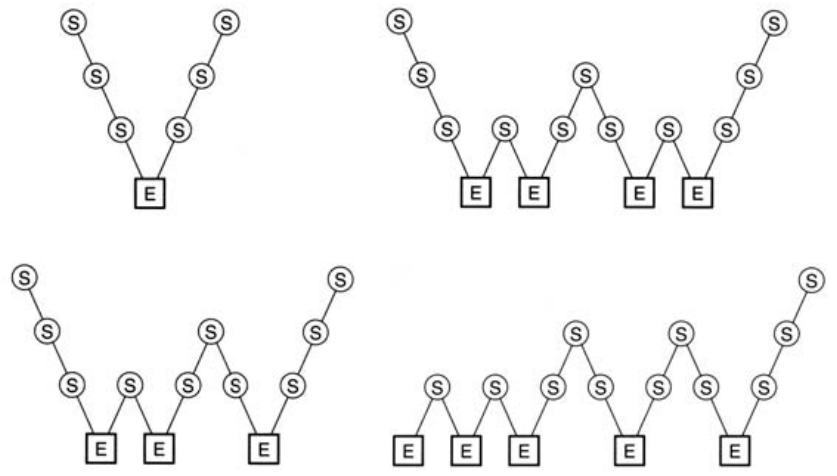
\includegraphics[width=8cm]{images/multigrid/cycles}\\
{\scriptsize Taken from \cite{tack10}: Different types of multigrid cycle with four grid levels: (top left) V-cycle, (top right) W-cycle,
(bottom left) F-cycle and (bottom right) full multigrid. ‘S’ denotes smoothing while ‘E’ denotes
exact coarse-grid solution.}
\end{center} 

Check Kaus BEcker syllabus!

\Literature: \cite{pisa85,tack10,gery10,mabl15,lopp14,tros01,moma05,yaba00,yavn06}
